\documentclass[conference]{IEEEtran}
\IEEEoverridecommandlockouts

\usepackage[utf8]{inputenc}
\usepackage[T1]{fontenc}
\usepackage{cite}
\usepackage{amsmath,amssymb,amsfonts}
\usepackage{dsfont}
\usepackage{graphicx}
\usepackage{textcomp}
\usepackage{xcolor}
\usepackage{booktabs}
\usepackage{multirow}
\usepackage{array}
\usepackage{url}
\usepackage{balance}

\graphicspath{{images/}{./images/}}

\def\BibTeX{{\rm B\kern-.05em{\sc i\kern-.025em b}\kern-.08em
    T\kern-.1667em\lower.7ex\hbox{E}\kern-.125emX}}

\begin{document}

\title{Reproducing a Synergistic Foundation-Conventional Pipeline for Mixed-Domain Semi-Supervised Medical Image Segmentation}

\author{\IEEEauthorblockN{Nguyen Huu Anh Tri}
\IEEEauthorblockA{Student ID: 23127130\\
Faculty of Information Technology\\
University of Science, VNU-HCM\\
Ho Chi Minh City, Vietnam\\
nhatri23@clc.fitus.edu.vn}
\and
\IEEEauthorblockN{Le Trung Kien}
\IEEEauthorblockA{Student ID: 23127075\\
Faculty of Information Technology\\
University of Science, VNU-HCM\\
Ho Chi Minh City, Vietnam\\
ltkien23@clc.fitus.edu.vn}
\and
\IEEEauthorblockN{Tran Hoai Thien Nhan}
\IEEEauthorblockA{Student ID: 23127238\\
Faculty of Information Technology\\
University of Science, VNU-HCM\\
Ho Chi Minh City, Vietnam\\
thtnhan23@clc.fitus.edu.vn}
}

\maketitle

\begin{abstract}
Large vision foundation models pretrained on massive datasets have demonstrated remarkable performance across various visual tasks. However, when applied to domain-specific applications such as semi-supervised medical image segmentation under domain shift, their strong prior knowledge may lead to overconfident predictions even when some of them are incorrect. These inaccurate pseudo-labels can accumulate during training, reducing the effectiveness of unlabeled data and limiting segmentation performance. In this work, we reproduce the SynFoC (Synergistic Training for Foundation and Conventional Models) framework, which jointly trains a foundation model and a conventional segmentation model to alleviate this issue. The conventional model, trained from scratch, helps correct the high-confidence errors made by the foundation model, while the foundation model provides reliable pseudo-labels that guide the conventional model during the early stages of training. The framework further employs consensus-divergence consistency regularization to encourage effective collaboration between the two models and improve training stability. We evaluate the reproduced implementation on four public multi-domain medical image segmentation datasets and report the experimental results obtained in our reproduction study. The implementation follows the original code released by the paper's authors at \url{https://github.com/MQinghe/SynFoC}.
\end{abstract}

\begin{IEEEkeywords}
medical image segmentation, semi-supervised learning, mixed-domain learning, foundation model, MedSAM, U-Net
\end{IEEEkeywords}


\section{Introduction}
Semi-supervised medical image segmentation (SSMIS) is an effective way to reduce the burden of manual annotation in medical imaging \cite{tarvainen2017mean,chen2021semi,yu2019uncertainty,grunberg2017annotating}. In practice, however, clinical data rarely follow a single distribution. Scanner settings, hospital protocols, and patient populations can all introduce domain shift, which makes unlabeled samples less reliable to exploit and often leads to unstable pseudo-labeling when the labeled set is small \cite{ma2024constructing}.

A common solution is to train a conventional segmentation model such as U-Net from scratch \cite{ronneberger2015u}. This remains attractive because it adapts well to the target task, but it is also sensitive to noisy pseudo-labels and can overfit the labeled domain when the distribution gap is large. Foundation models offer another option. SAM and MedSAM are able to transfer strong segmentation priors from large-scale pretraining \cite{kirillov2023segment,ma2024segment}, yet those priors are not always beneficial under a new medical target domain. In mixed-domain semi-supervision, they may produce confident predictions that are still wrong, and such errors can accumulate during training \cite{ma2024constructing}.

This motivates our reproduction of SynFoC (Synergistic Training for Foundation and Conventional Models), a framework that trains a foundation model and a conventional model together. In the reproduced setting, MedSAM acts as the foundation branch and U-Net acts as the conventional branch. The conventional model, trained from scratch, helps correct the high-confidence errors made by the foundation model, while the foundation model provides reliable pseudo-labels that guide the conventional model during the early stages of training. The two branches are not treated as fixed teacher and student in a one-way pipeline; instead, they are trained synergistically so that each can compensate for the other at different stages. We follow the released training code and summarize the results from the completed logs rather than proposing a new method \cite{ma2024constructing}.

The framework uses self-mutual confidence (SMC) to determine how pseudo-labels from the two branches should be combined, and consensus-divergence consistency regularization (CDCR) to apply different constraints to agreement and disagreement regions. These mechanisms encourage effective collaboration between the two models and improve training stability under domain shift \cite{ma2024constructing}.

Our contributions are:
\begin{itemize}
    \item We reproduce the SynFoC training framework for mixed-domain semi-supervised medical image segmentation.
    \item We summarize the roles of SMC and CDCR in the released training pipeline using the available logs.
    \item We report the completed reproduced experiments on four public datasets and compare the logged results with the original paper where the settings are comparable.
\end{itemize}


\section{Related Work}
\subsection{Semi-Supervised Medical Image Segmentation}
SSMIS methods generally use either pseudo-labeling or consistency regularization. Pseudo-labeling assigns labels to unlabeled images and uses them as supervision in later optimization \cite{lee2013pseudo}. Consistency-based methods encourage stable predictions under input, feature, or network perturbations \cite{chen2021semi}. Mean Teacher, for example, updates a teacher network as an exponential moving average of a student network and uses the teacher to supervise unlabeled samples \cite{tarvainen2017mean,yu2019uncertainty}. More recent segmentation methods such as FixMatch-style training, SS-Net, BCP, CauSSL, and ABD improve pseudo-label filtering, perturbation design, or copy-paste training \cite{sohn2020fixmatch,upretee2022fixmatchseg,wu2022exploring,bai2023bidirectional,miao2023caussl,chi2024adaptive}. These methods are effective, but many assume that labeled and unlabeled data are sampled from similar distributions.

\subsection{Medical Image Segmentation under Domain Shift}
Domain shift is common in medical imaging. MiDSS is more challenging than standard SSMIS because the labeled data come from one domain, whereas unlabeled data come from multiple unknown domains \cite{ma2024constructing}. Intermediate-sample strategies have been used to bridge distribution gaps in this setting, but conventional models can still be fragile when labeled data are extremely limited or when the labeled domain is far from the unlabeled domains.

\subsection{Foundation Models for Medical Segmentation}
SAM introduced promptable general segmentation at scale \cite{kirillov2023segment}. MedSAM further adapts SAM to medical images using a large collection of medical image-mask pairs \cite{ma2024segment}. Since fully fine-tuning such large models is expensive, parameter-efficient strategies such as adapters and low-rank adaptation (LoRA) are commonly used \cite{hu2021lora,zhang2023customized}. SemiSAM, H-SAM, and CPC-SAM explore how SAM-like models can support semi-supervised medical segmentation \cite{zhang2023semisam,cheng2024unleashing,miao2024cross}. Compared with methods that keep the foundation model fixed or use it only as a static teacher, the reproduced SynFoC pipeline trains the foundation model and the conventional model jointly and lets them influence each other during optimization.


\section{Method}
\subsection{Problem Formulation}
Let $\mathcal{L}=\{(X_i,Y_i)\}_{i=1}^{N}$ denote the labeled set and $\mathcal{U}=\{U_i\}_{i=1}^{M}$ denote the unlabeled set, where $M \geq N$. Each image is $X_i,U_i\in\mathbb{R}^{W\times H\times L}$, and each mask is $Y_i\in\{0,1,\ldots,C\}^{W\times H}$, where class 0 is background. Training data are sampled from $K$ domains. In MiDSS, $\mathcal{L}$ comes from one domain, while $\mathcal{U}$ contains samples from multiple domains without requiring domain labels \cite{ma2024constructing}.

The base semi-supervised training follows a Mean Teacher-style design \cite{tarvainen2017mean}. For an unlabeled image $U$, weak and strong augmentations generate $U_w$ and $U_s$. A teacher model predicts a probability map $\hat{P}_w$ on $U_w$, and the pseudo-label is $\hat{Q}_w=\arg\max(\hat{P}_w)$ \cite{lee2013pseudo}. To connect labeled and unlabeled domains, an intermediate sample is generated by copy-paste:
\begin{equation}
\begin{gathered}
U_c=X_w\odot M+U_s\odot(\mathbf{1}-M),\\
\hat{Q}_c=Y_w\odot M+\hat{Q}_w\odot(\mathbf{1}-M),
\end{gathered}
\label{eq:copy_paste}
\end{equation}
where $M\in\{0,1\}^{W\times H}$ is the pasted region mask and $\odot$ denotes element-wise multiplication.

\subsection{Overall Pipeline}
Fig.~\ref{fig:framework} shows the reproduced synergistic training pipeline. The two student models are U-Net, denoted $f^{UT}$, and MedSAM, denoted $f^{MS}$. Each has a corresponding teacher model, $\hat{f}^{UT}$ and $\hat{f}^{MS}$, updated by exponential moving average. For MedSAM, LoRA is applied to reduce the adaptation cost while preserving pretrained knowledge \cite{hu2021lora}.

\begin{figure*}[t]
\centering
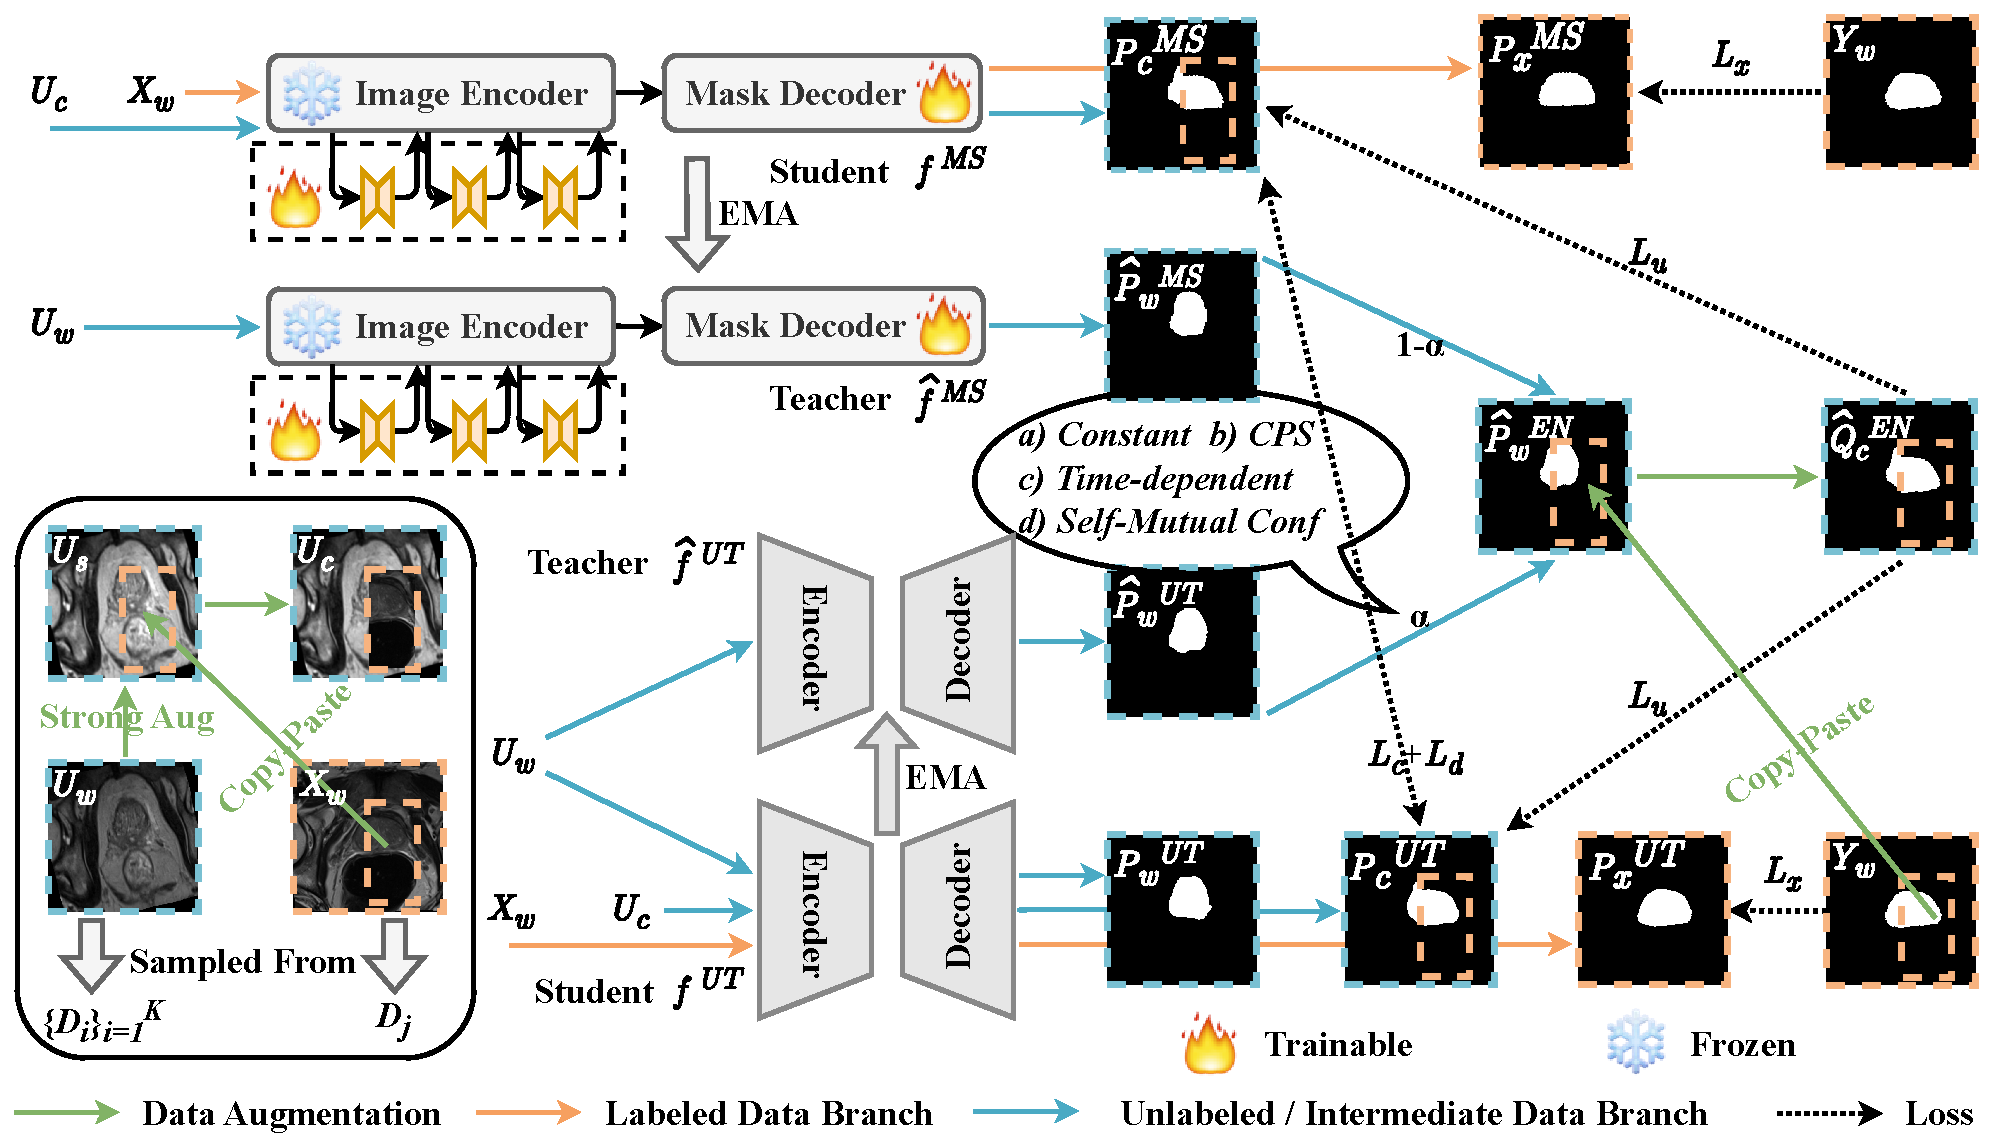
\includegraphics[width=0.86\textwidth]{Framework.pdf}
\caption{Reproduced SynFoC pipeline. U-Net and MedSAM both produce pseudo-labels, and the two branches are trained jointly so that each can correct the other at different stages.}
\label{fig:framework}
\end{figure*}

The supervised losses of U-Net and MedSAM are computed independently on labeled images. For unlabeled images, the teacher predictions are first combined by an instance-wise ensemble ratio $\alpha$ to produce an ensembled probability map:
\begin{equation}
\hat{P}^{EN}_w=\alpha\hat{P}^{UT}_w+(1-\alpha)\hat{P}^{MS}_w,
\label{eq:ensemble}
\end{equation}
where $\alpha$ controls the contribution from U-Net. The ensembled pseudo-label is then inserted into the copy-paste sample $U_c$ to supervise both student branches, while consensus-divergence consistency regularization is applied to the predictions on $U_c$. The total objective is
\begin{equation}
L_{total}=L_x+\lambda(t)(L_u+L_c+L_d),
\label{eq:total_loss}
\end{equation}
where $L_x$ is the supervised loss, $L_u$ is the unsupervised pseudo-label loss, $L_c$ and $L_d$ are the consensus and divergence regularizers, and
\begin{equation}
\lambda(t)=e^{-5(1-t/t_{max})^2}
\label{eq:lambda}
\end{equation}
is the Gaussian ramp-up weight used during training.

\subsection{Self-Mutual Confidence}
The ensemble ratio should reflect whether U-Net has become reliable for a particular unlabeled instance. Let $Q^{UT}_w=\arg\max(P^{UT}_w)$, $\hat{Q}^{UT}_w=\arg\max(\hat{P}^{UT}_w)$, and $\hat{Q}^{MS}_w=\arg\max(\hat{P}^{MS}_w)$. SMC measures the reliability of the U-Net prediction from two perspectives.

\textbf{Self-confidence.} Self-confidence $\Phi^{self}$ measures the consistency between the U-Net student and teacher predictions:
\begin{equation}
\Phi^{self}=\frac{1}{C}\sum_{i=1}^{C}\frac{2\left|\mathds{1}(Q^{UT}_w=i)\cap\mathds{1}(\hat{Q}^{UT}_w=i)\right|}{\left|\mathds{1}(Q^{UT}_w=i)\right|+\left|\mathds{1}(\hat{Q}^{UT}_w=i)\right|},
\label{eq:self_conf}
\end{equation}
where $\mathds{1}(\cdot)$ is the indicator function and $|\cdot|$ counts the number of pixels in the corresponding binary mask.

\textbf{Mutual confidence.} Mutual confidence $\Phi^{mut}$ measures the agreement between the U-Net teacher and the MedSAM teacher:
\begin{equation}
\Phi^{mut}=\frac{1}{C}\sum_{i=1}^{C}\frac{2\left|\mathds{1}(\hat{Q}^{MS}_w=i)\cap\mathds{1}(\hat{Q}^{UT}_w=i)\right|}{\left|\mathds{1}(\hat{Q}^{MS}_w=i)\right|+\left|\mathds{1}(\hat{Q}^{UT}_w=i)\right|}.
\label{eq:mut_conf}
\end{equation}
When both values are high, the U-Net pseudo-label is treated as reliable and should receive a larger ensemble weight. Therefore, the instance-wise ratio is defined as
\begin{equation}
\alpha=\Phi^{self}\times\Phi^{mut}.
\label{eq:alpha}
\end{equation}

After computing $\alpha$, we obtain the ensembled pseudo-label $\hat{Q}^{EN}_w=\arg\max(\hat{P}^{EN}_w)$ and form the mixed pseudo-label
\begin{equation}
\hat{Q}^{EN}_c=Y_w\odot M+\hat{Q}^{EN}_w\odot(\mathbf{1}-M).
\label{eq:ensemble_copy_paste}
\end{equation}
We further keep only confident unlabeled regions using the mask
\begin{equation}
\begin{gathered}
W^{EN}_w=\mathds{1}(\max(\hat{P}^{EN}_w)\geq \tau),\\
W^{EN}_c=M+W^{EN}_w\odot(\mathbf{1}-M),
\end{gathered}
\label{eq:confidence_mask}
\end{equation}
where $\tau=0.95$ is the confidence threshold. The unsupervised loss on the copy-paste sample is then
\begin{equation}
\begin{aligned}
L_u={}&L_{ce}(\hat{Q}^{EN}_c,P^{UT}_c,W^{EN}_c)+L_{dice}(\hat{Q}^{EN}_c,P^{UT}_c,W^{EN}_c)\\
&+L_{ce}(\hat{Q}^{EN}_c,P^{MS}_c,W^{EN}_c)+L_{dice}(\hat{Q}^{EN}_c,P^{MS}_c,W^{EN}_c),
\end{aligned}
\label{eq:unsup_loss}
\end{equation}
where $P^{UT}_c$ and $P^{MS}_c$ are the student predictions on $U_c$.

\subsection{Consensus-Divergence Consistency Regularization}
SMC improves pseudo-label quality, but the two models can still disagree in difficult regions. CDCR separates the student predictions on $U_c$ into consensus and divergence regions:
\begin{equation}
\begin{gathered}
M_c=\mathds{1}(Q^{UT}_c=Q^{MS}_c),\\
M_d=\mathbf{1}-M_c,
\end{gathered}
\label{eq:cdcr_masks}
\end{equation}
where $Q^{UT}_c=\arg\max(P^{UT}_c)$ and $Q^{MS}_c=\arg\max(P^{MS}_c)$. Fig.~\ref{fig:modules} illustrates the SMC and CDCR modules.

\begin{figure}[t]
\centering
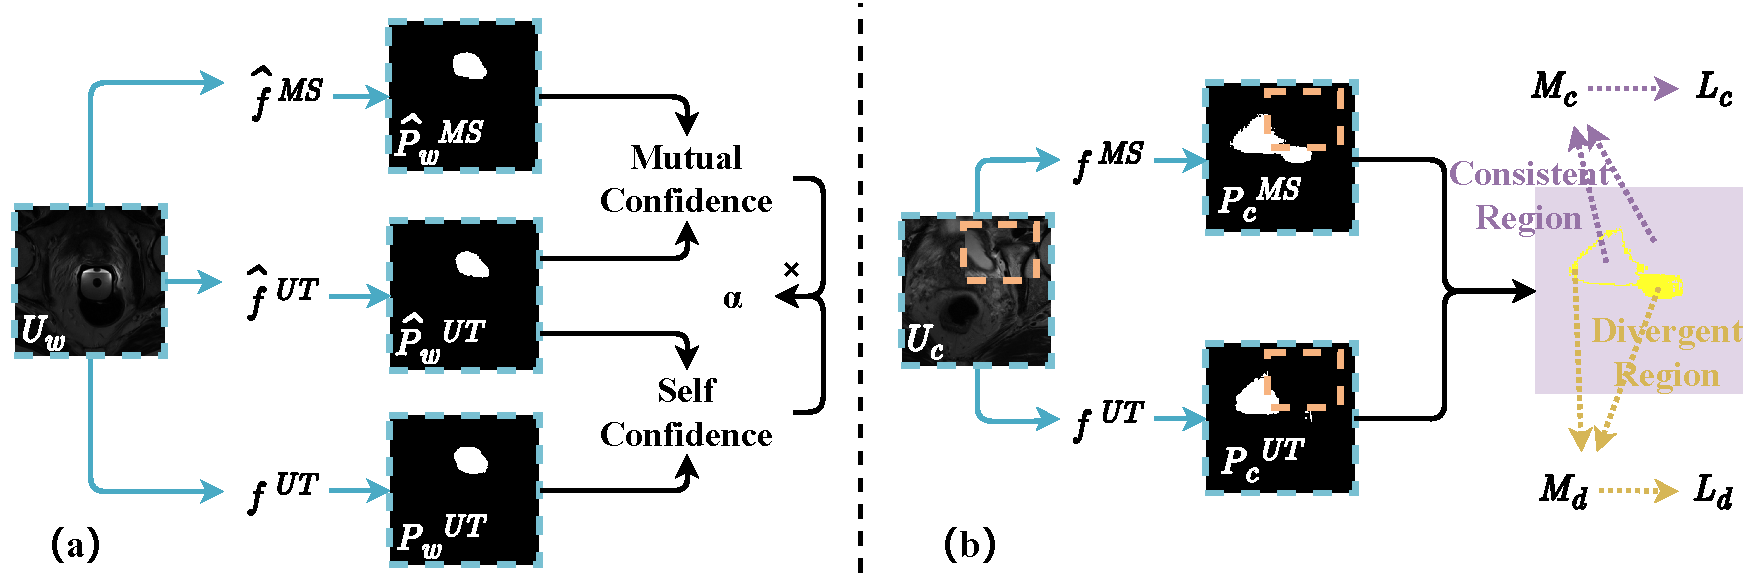
\includegraphics[width=0.95\linewidth]{modules.pdf}
\caption{SMC estimates pseudo-label reliability, while CDCR applies different constraints to agreement and disagreement regions.}
\label{fig:modules}
\end{figure}

\textbf{Consensus regularization.} In consensus regions, the models are encouraged to make confident predictions by minimizing entropy:
\begin{equation}
L_c=-\frac{1}{2S}\sum\left[(P^{UT}_c\log P^{UT}_c)\odot M_c+(P^{MS}_c\log P^{MS}_c)\odot M_c\right],
\label{eq:consensus_loss}
\end{equation}
where $S=W\times H\times C$. In practice, interpolation is used wherever the resolutions of U-Net and MedSAM predictions need to be aligned.

\textbf{Divergence regularization.} In divergence regions, the models are encouraged to reduce prediction discrepancies through mean squared error:
\begin{equation}
L_d=\frac{1}{S}\sum \mathrm{MSE}(P^{UT}_c,P^{MS}_c)\odot M_d.
\label{eq:divergence_loss}
\end{equation}
This separation lets the method reward agreement where the two branches already align and focus discrepancy reduction on the regions where their predictions differ most.


\section{Experiments}
\subsection{Datasets and Metrics}
This report summarizes the completed training logs found under the reproduced \texttt{SyncRepo/model} directory. The Prostate dataset is a multi-site T2-weighted MRI dataset for prostate segmentation, collected from six sources: RUNMC, BMC, HCRUDB, UCL, BIDMC, and HK \cite{liu2020shape}. Slices are resized to $384\times384$. The Fundus dataset contains images from four centers for optic cup and optic disc segmentation \cite{wang2020dofe}. The region of interest is resized to $256\times256$.

The M\&Ms dataset is a cardiac MRI dataset collected from four scanner vendors \cite{campello2021multi}. We evaluate the left ventricle (LV), myocardium (MYO), and right ventricle (RV) segmentation targets, with each 2D slice resized to $288\times288$. The BUSI dataset contains breast ultrasound images \cite{al2020dataset}. Following the reproduced setting, the normal category is excluded because it has no tumor segmentation target, and the benign and malignant cases are treated as two domains. Images are resized to $256\times256$.

Our comparisons are guided by earlier work on semi-supervised learning, pseudo-labeling, and consistency regularization \cite{tarvainen2017mean,lee2013pseudo,sohn2020fixmatch,chen2021semi}. Mixed-domain settings are also important because they expose the weakness of methods that assume a single data distribution \cite{ma2024constructing}. Foundation-based adaptation further motivates the use of MedSAM as the stronger prior branch in this reproduction study \cite{kirillov2023segment,ma2024segment}.

We evaluate with Dice Similarity Coefficient (DSC), Jaccard Index, 95\% Hausdorff Distance (95HD), and Average Surface Distance (ASD). Higher DSC and Jaccard are better, while lower 95HD and ASD are better. The SynFoC rows are taken from the best average-DSC checkpoints recorded in each \texttt{log.txt} file.

\subsection{Implementation Details}
The reproduced analysis distinguishes between the original paper setting and the completed logs stored under \texttt{SyncRepo/model}. In the original paper, SynFoC is trained on an NVIDIA GeForce RTX 3090 GPU. U-Net is optimized by stochastic gradient descent with momentum 0.9, weight decay 0.0001, and initial learning rate 0.03. MedSAM uses the ViT-B backbone with input size $512\times512$, AdamW with initial learning rate 0.0001, $\beta_1=0.9$, $\beta_2=0.999$, weight decay 0.1, and LoRA rank 4. The confidence-threshold ablation in the original paper selects $\tau=0.95$ as the best setting. The original label regime uses 20 labeled samples for Prostate and Fundus, 5 for M\&Ms, and 64 or 129 for BUSI. Except for M\&Ms, the batch size is 8 with an even split between labeled and unlabeled samples; the M\&Ms batch size is reduced to 4 because only 5 labeled samples are used. Prostate and M\&Ms are trained for 60,000 iterations, while Fundus and BUSI are trained for 30,000 iterations. In contrast, the completed reproduced runs currently available in \texttt{SyncRepo/model} use domain-1 training logs with 40 labeled samples, \texttt{--AdamW}, \texttt{--warmup}, \texttt{--model MedSAM}, threshold 0.95, LoRA rank 4, input size 512, and an effective labeled/unlabeled batch split of 4/4 in the released logs.

\subsection{Logged Results Across Four Datasets}
The baseline rows are retained as contextual reference values where they were already available in the previous report. Since the reproduced logs use 40 labeled samples from domain 1, cross-method comparisons should be interpreted as contextual rather than as a strict identical-label setting. This section focuses on the completed runs stored in the repository and on how those runs compare with the originally published numbers when the label regime is close enough to make the comparison meaningful. When the setting is too different for a strict one-to-one comparison, we report the reproduced numbers directly and explain the mismatch instead of forcing a conclusion.

Table~\ref{tab:prostate_results} reports Prostate results from the logged domain-1 run. The reproduced U-Net side obtains the best logged average performance, with 88.73\% DSC, 81.30\% Jaccard, 9.65 95HD, and 4.17 ASD.

\begin{table}[!htbp]
\centering
\caption{Comparison on the Prostate dataset using the reproduced domain-1 run.}
\label{tab:prostate_results}
\resizebox{\columnwidth}{!}{%
\begin{tabular}{lcccccccccc}
\toprule
Method & RUNMC & BMC & HCRUDB & UCL & BIDMC & HK & DSC $\uparrow$ & Jaccard $\uparrow$ & 95HD $\downarrow$ & ASD $\downarrow$ \\
\midrule
SupOnly & 22.11 & 21.81 & 19.60 & 13.87 & 18.16 & 26.98 & 20.42 & 15.63 & 118.15 & 79.70 \\
UA-MT \cite{yu2019uncertainty} & 19.09 & 13.66 & 16.07 & 37.30 & 15.23 & 11.22 & 18.76 & 13.44 & 127.59 & 85.76 \\
FixMatch \cite{sohn2020fixmatch} & 81.69 & 65.27 & 53.70 & 70.40 & 10.20 & 81.22 & 60.41 & 52.53 & 49.47 & 28.83 \\
BCP \cite{bai2023bidirectional} & 64.79 & 62.46 & 50.49 & 55.08 & 63.31 & 57.64 & 58.96 & 48.74 & 56.81 & 27.77 \\
ABD \cite{chi2024adaptive} & 53.10 & 62.28 & 9.17 & 59.22 & 51.92 & 22.19 & 42.98 & 32.35 & 75.73 & 47.17 \\
SymGD \cite{ma2024constructing} & 88.34 & 83.26 & 83.99 & 85.45 & 42.03 & 78.02 & 76.85 & 67.88 & 39.02 & 21.08 \\
SAMed \cite{zhang2023customized} & 63.67 & 65.62 & 65.25 & 68.65 & 48.83 & 75.31 & 64.56 & 53.49 & 35.85 & 15.83 \\
SemiSAM \cite{zhang2023semisam} & 78.07 & 67.16 & 76.49 & 69.25 & 65.97 & 69.76 & 71.12 & 59.69 & 28.19 & 12.61 \\
CPC-SAM \cite{miao2024cross} & 77.23 & 66.46 & 66.98 & 76.79 & 79.71 & 75.42 & 73.77 & 62.85 & 31.08 & 13.16 \\
SynFoC U-Net & \textbf{88.49} & \textbf{90.26} & 89.37 & \textbf{89.77} & 85.75 & \textbf{88.75} & \textbf{88.73} & \textbf{81.30} & \textbf{9.65} & \textbf{4.17} \\
SynFoC MedSAM & 86.49 & 89.82 & \textbf{89.81} & 89.61 & \textbf{86.56} & 86.67 & 88.16 & 80.49 & 9.78 & 4.35 \\
\bottomrule
\end{tabular}}
\end{table}

Table~\ref{tab:fundus_results} reports Fundus results. The reproduced MedSAM-side model reaches the best average performance among all compared methods, with 89.73\% DSC and 82.27\% Jaccard. It also reduces the average 95HD to 6.77 and ASD to 3.22.

\begin{table}[!htbp]
\centering
\caption{Comparison on the Fundus dataset using the reproduced domain-1 run. Domain columns report optic cup / optic disc DSC.}
\label{tab:fundus_results}
\resizebox{\columnwidth}{!}{%
\begin{tabular}{lcccccccc}
\toprule
Method & Domain 1 & Domain 2 & Domain 3 & Domain 4 & DSC $\uparrow$ & Jaccard $\uparrow$ & 95HD $\downarrow$ & ASD $\downarrow$ \\
\midrule
SupOnly & 59.54 / 73.89 & 71.28 / 74.23 & 50.87 / 64.29 & 35.61 / 63.30 & 61.63 & 52.65 & 48.28 & 28.86 \\
UA-MT \cite{yu2019uncertainty} & 59.35 / 78.46 & 63.08 / 74.45 & 35.24 / 47.73 & 36.18 / 55.43 & 56.24 & 47.00 & 48.64 & 31.35 \\
FixMatch \cite{sohn2020fixmatch} & 81.18 / 91.29 & 72.04 / 87.60 & 80.41 / 92.95 & 74.58 / 87.07 & 83.39 & 73.48 & 11.77 & 5.60 \\
BCP \cite{bai2023bidirectional} & 71.65 / 91.10 & 77.19 / 92.00 & 72.63 / 90.77 & 77.67 / 91.42 & 83.05 & 73.66 & 11.05 & 5.80 \\
ABD \cite{chi2024adaptive} & 73.92 / 79.71 & 65.19 / 90.96 & 77.61 / 86.11 & 74.79 / 86.72 & 79.38 & 69.28 & 13.99 & 8.14 \\
SymGD \cite{ma2024constructing} & 83.71 / 92.96 & 80.47 / 89.93 & 84.18 / 92.97 & 83.71 / 93.38 & 87.66 & 79.10 & 8.21 & 3.89 \\
SAMed \cite{zhang2023customized} & 71.00 / 93.53 & 81.77 / 90.04 & 82.07 / 92.25 & 71.62 / 93.14 & 84.47 & 75.69 & 9.83 & 5.25 \\
SemiSAM \cite{zhang2023semisam} & 83.70 / 93.21 & 72.40 / 87.72 & 81.39 / 92.11 & 79.17 / 91.10 & 85.10 & 75.50 & 9.48 & 4.60 \\
CPC-SAM \cite{miao2024cross} & 75.99 / 94.34 & 80.10 / 93.08 & 83.19 / 92.81 & 83.43 / 93.20 & 87.02 & 78.65 & 8.50 & 4.24 \\
SynFoC U-Net & 88.68 / \textbf{97.33} & 78.82 / 90.61 & 86.09 / 92.51 & 86.37 / 91.18 & 88.95 & 81.13 & 6.93 & 3.37 \\
SynFoC MedSAM & \textbf{89.39} / 96.97 & 79.06 / 92.77 & \textbf{86.60} / 92.79 & \textbf{88.71} / 91.58 & \textbf{89.73} & \textbf{82.27} & \textbf{6.77} & \textbf{3.22} \\
\bottomrule
\end{tabular}}
\end{table}

Table~\ref{tab:mnms_results} reports the M\&Ms run. The U-Net side gives the best logged average DSC at 81.98\%, while the MedSAM side obtains a lower ASD of 3.92. This indicates that the conventional model reaches stronger overlap in the final selected checkpoint, whereas the foundation model still produces compact boundary errors.

\begin{table}[!htbp]
\centering
\caption{Logged SynFoC results on the M\&Ms dataset. Vendor columns report LV / MYO / RV DSC.}
\label{tab:mnms_results}
\resizebox{\columnwidth}{!}{%
\begin{tabular}{lcccccccc}
\toprule
Method & Vendor A & Vendor B & Vendor C & Vendor D & DSC $\uparrow$ & Jaccard $\uparrow$ & 95HD $\downarrow$ & ASD $\downarrow$ \\
\midrule
SynFoC U-Net & 90.49 / 81.86 / 79.72 & 88.65 / 82.56 / \textbf{83.69} & 86.68 / \textbf{76.23} / \textbf{68.92} & 87.24 / \textbf{79.29} / \textbf{78.44} & \textbf{81.98} & \textbf{72.80} & \textbf{7.82} & 4.42 \\
SynFoC MedSAM & \textbf{90.60} / 81.46 / 78.85 & 87.93 / 81.33 / 80.35 & \textbf{86.72} / 75.36 / 67.89 & 87.05 / 77.32 / 76.89 & 80.98 & 71.54 & 8.13 & \textbf{3.92} \\
\bottomrule
\end{tabular}}
\end{table}

Table~\ref{tab:busi_results} reports the BUSI run. MedSAM has the best logged average performance, reaching 62.84\% DSC, 53.01\% Jaccard, 42.38 95HD, and 19.38 ASD. The domain-level gap is large: the benign domain is segmented much more accurately than the malignant domain, suggesting that the malignant subset is the harder cross-domain case in this run.

\begin{table}[!htbp]
\centering
\caption{Logged SynFoC results on the BUSI dataset.}
\label{tab:busi_results}
\resizebox{\columnwidth}{!}{%
\begin{tabular}{lcccccc}
\toprule
Method & Benign & Malignant & DSC $\uparrow$ & Jaccard $\uparrow$ & 95HD $\downarrow$ & ASD $\downarrow$ \\
\midrule
SynFoC U-Net & 75.67 & 23.55 & 49.61 & 42.66 & 53.41 & 27.69 \\
SynFoC MedSAM & \textbf{76.86} & \textbf{48.83} & \textbf{62.84} & \textbf{53.01} & \textbf{42.38} & \textbf{19.38} \\
\bottomrule
\end{tabular}}
\end{table}

Fig.~\ref{fig:visuals} provides qualitative examples from Prostate, Fundus, M\&Ms, and BUSI. The visual results support the quantitative trend: the synergistic pipeline produces more complete and stable segmentation masks in cross-domain samples.

\begin{figure}[!htbp]
\centering
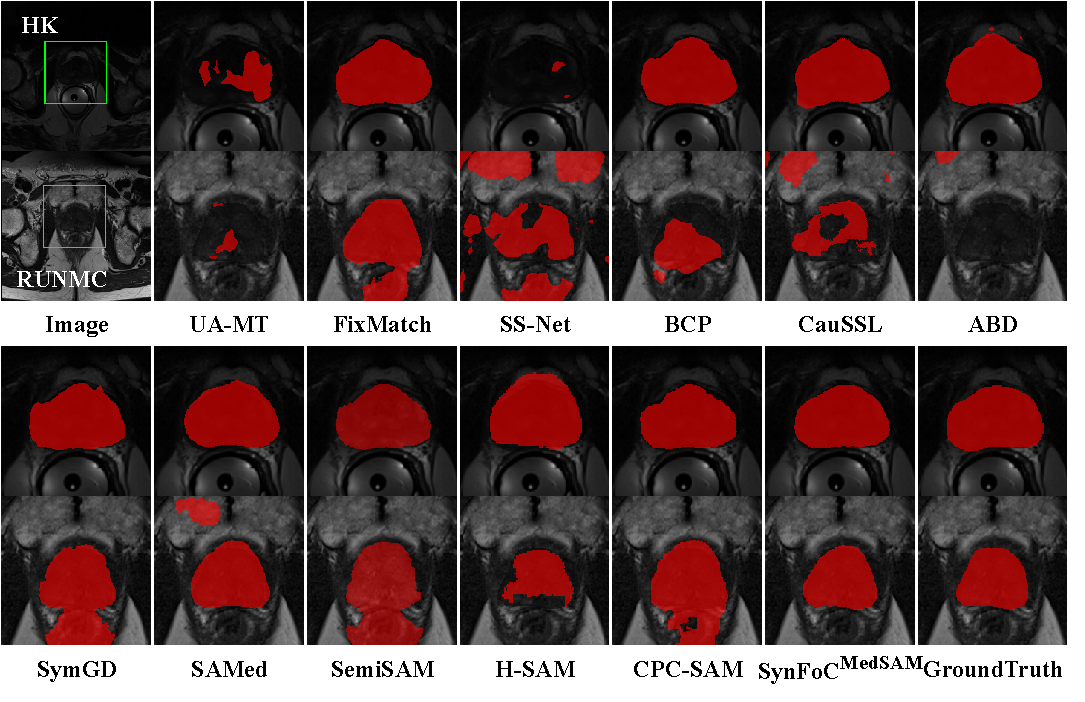
\includegraphics[width=0.98\columnwidth]{prostate_img.pdf}
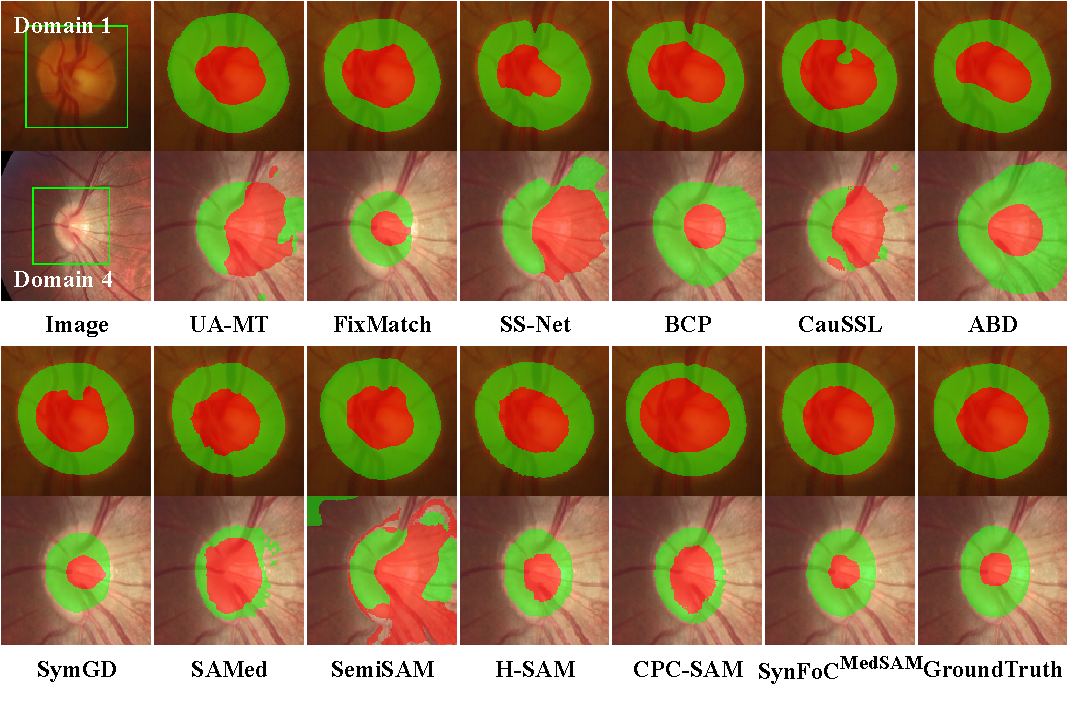
\includegraphics[width=0.98\columnwidth]{fundus_img.pdf}
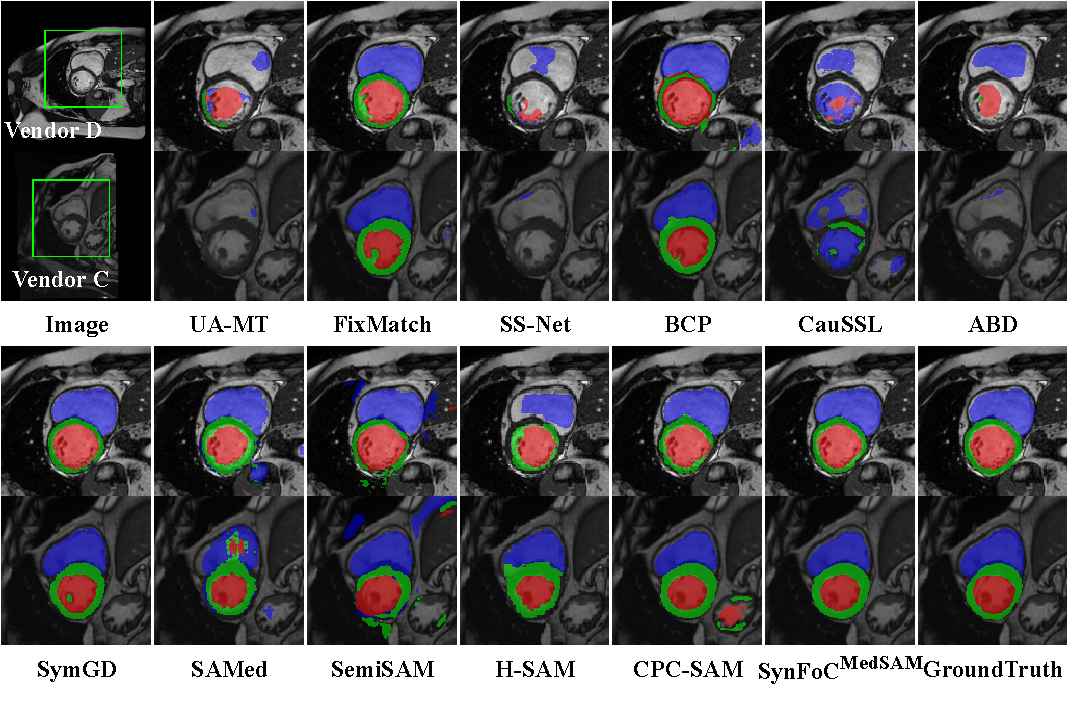
\includegraphics[width=0.98\columnwidth]{MNMS_img.pdf}
\includegraphics[width=0.98\columnwidth]{BUSI_img.pdf}
\caption{Qualitative visualizations on Prostate, Fundus, M\&Ms, and BUSI datasets.}
\label{fig:visuals}
\end{figure}

\subsection{Comparison with the Original Paper}
Table~\ref{tab:original_vs_reproduced} compares the headline SynFoC averages reported in the original paper tables with the best averages extracted from the completed reproduced logs. The comparison is only approximate because the reproduced logs use 40 labeled samples from domain 1, whereas the original paper reports dataset-specific label regimes.

\begin{table}[!htbp]
\centering
\caption{Original paper versus reproduced logged best average DSC. BUSI is not directly comparable because the original paper reports 64-label and 129-label settings, while the reproduced logs use 40 labeled samples from domain 1.}
\label{tab:original_vs_reproduced}
\resizebox{\columnwidth}{!}{%
\begin{tabular}{lccc}
\toprule
Dataset & Original paper & Reproduced log & Comment \\
\midrule
Prostate & 87.16 (MedSAM) & 88.73 (U-Net) & different winner; reproduced log higher \\
Fundus & 88.60 (MedSAM) & 89.73 (MedSAM) & same winner; reproduced log higher \\
M\&Ms & 80.84 (MedSAM) & 81.98 (U-Net) & different winner; reproduced log higher \\
BUSI & 74.75 (MedSAM, 129 labels) & 62.84 (MedSAM) & different label regime \\
\bottomrule
\end{tabular}}
\end{table}


\section{Discussion}
The version-2 logs reinforce the main motivation of SynFoC: U-Net and MedSAM contribute differently across mixed-domain datasets, so a joint pipeline is more reliable than assuming one branch is always stronger. On Prostate and M\&Ms, the reproduced U-Net branch reaches the best average DSC, while on Fundus and BUSI, the MedSAM branch gives the better overall averages. This pattern is consistent with the idea that the stronger pseudo-label source depends on both the dataset characteristics and the training stage.

The qualitative figures also support the quantitative results. Across the four datasets, the reproduced masks are generally more complete on target structures when the two branches agree, while disagreement regions remain the main source of boundary errors. This makes the self-mutual confidence rule and the consensus-divergence consistency objective useful not only as optimization details, but also as practical mechanisms for handling cross-domain instability.

The current report still has several limitations. First, the conclusions are drawn from the completed logged runs with 40 labeled samples from domain 1, so comparisons with published baselines should be interpreted as contextual rather than strictly matched settings. Second, the analysis is based on the best recorded checkpoints in the available logs, not on repeated runs with statistical significance testing. Third, this work is a reproduction study, so it does not yet propose a new architectural extension beyond the released SynFoC pipeline. Future work should validate the stability of the reproduced results across multiple seeds and then explore stronger uncertainty estimation, more robust prompt generation, or lighter adaptation strategies for the foundation branch.


\section{Conclusion}
This report reorganizes the reproduced SynFoC study into the intended IEEE paper structure and summarizes completed results on four public medical image segmentation datasets. The reproduced SynFoC pipeline combines U-Net and MedSAM through self-mutual confidence pseudo-label integration and consensus-divergence consistency regularization, allowing the two branches to complement each other under mixed-domain semi-supervision. The logged results show that the stronger branch varies by dataset, which supports the central motivation for synergistic training. Overall, the manuscript now presents the reproduced experiments, qualitative figures, discussion, and conclusion as separate sections in a cleaner submission-ready layout while clarifying the relationship between the original paper settings and the reproduced SyncRepo logs.


\balance
\bibliographystyle{IEEEtran}
\bibliography{references}

\end{document}
